% \begin{figure*}[ht]
%   \adjustbox{valign=t}{
%   \begin{minipage}{0.55\linewidth}
%   \begin{subfigure}{\linewidth}
%     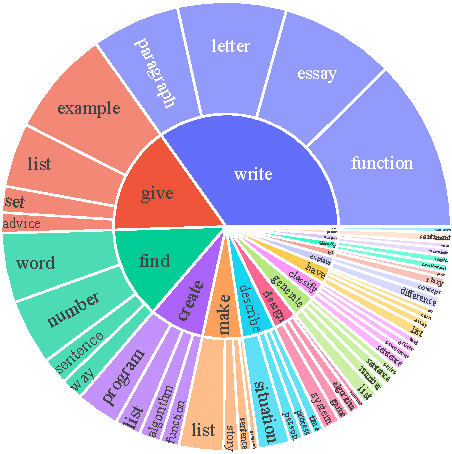
\includegraphics[width=\linewidth]{figures/instruction_sunburst_v2.pdf}
%     \caption{The top-20 most common root verbs (inner circle) and their top-4 direct noun objects (outer circle) in the generated instructions. Despite their diversity, the instructions shown here only account for 14\% of all the generated instructions because many instructions (e.g., ``Classify whether the user is satisfied with the service.'') do not contain such a verb-noun structure.}
%     \label{subfig:key-a}
%   \end{subfigure}\hfill
%   \end{minipage}
%   }
%   \hfill
%   \adjustbox{valign=t}{
%   \begin{minipage}{0.41\linewidth}
%     \vspace{10pt}
%     % \begin{subfigure}{0.475\linewidth}
%     %   \includegraphics[width=\linewidth]{figures/instruction_sunburst.pdf}
%     %   \caption{}\label{subfig:key-b}
%     % \end{subfigure}\hfill
%     \begin{subfigure}{0.95\linewidth}
%       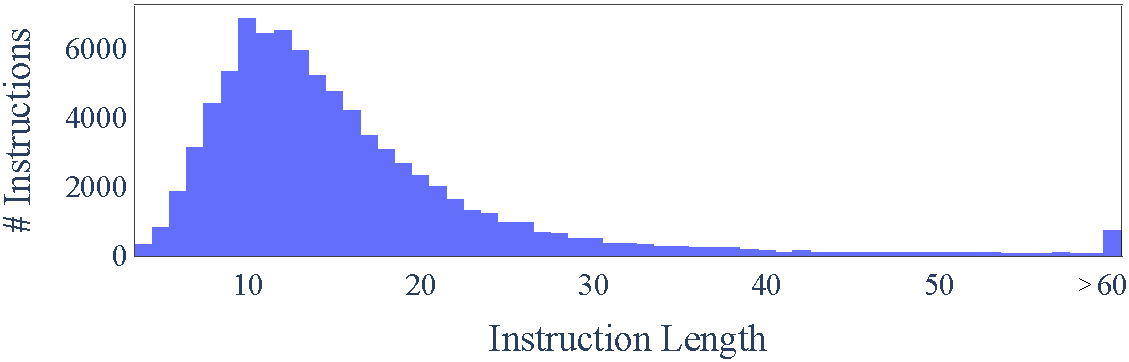
\includegraphics[width=\linewidth]{figures/instruction_length.pdf}
%       \caption{Distribution of instruction length (words)}\label{subfig:key-c}
%     \end{subfigure}
%     \medskip
%     \begin{subfigure}{0.95\linewidth}
%       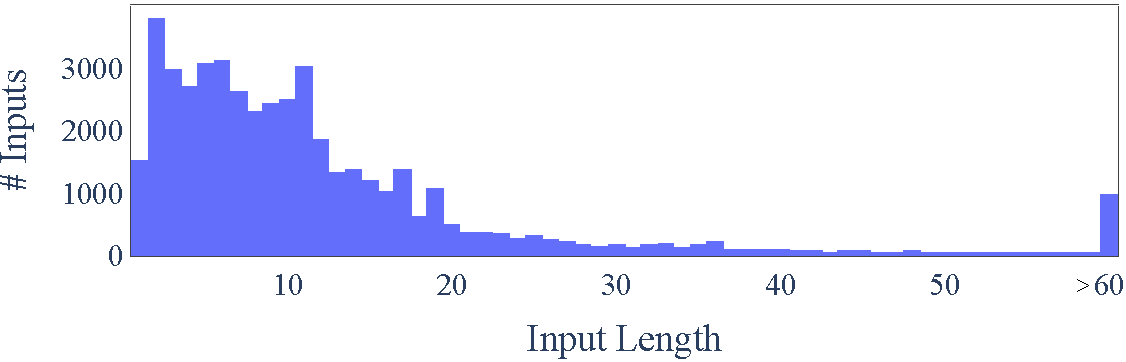
\includegraphics[width=\linewidth]{figures/input_length.pdf}
%       \caption{Distribution of non-empty input length (words)}\label{subfig:key-d}
%     \end{subfigure}\hfill
%     \begin{subfigure}{0.95\linewidth}
%       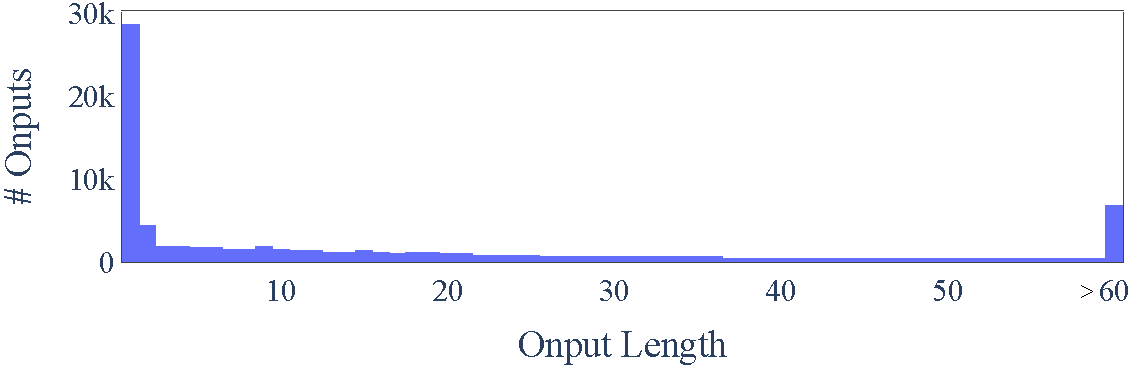
\includegraphics[width=\linewidth]{figures/output_length.pdf}
%       \caption{Distribution of output length (words)}\label{subfig:key-e}
%     \end{subfigure}\hfill
%   \end{minipage}
%   }
%   \caption{Distribution statistics of the generated instruction data. \todo{Make the font bigger. Make them different figures. Include a figure for the distance between generated instructions and their most similar seed tasks.}
%   % \daniel{state the unit of measurement (``token''?)} 
%   }
%   \label{fig:generated_data_distribution}
% \end{figure*}



\begin{figure*}[ht]
  \adjustbox{valign=t}{
  \begin{minipage}{0.55\linewidth}
    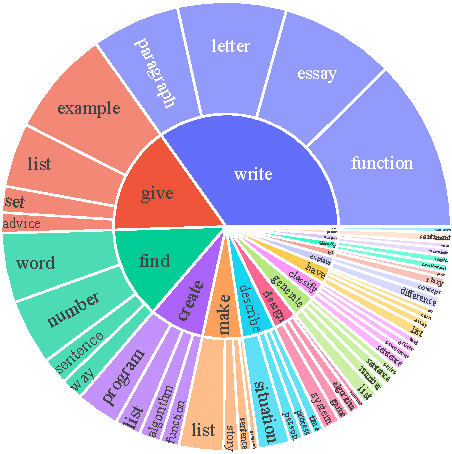
\includegraphics[width=0.98\linewidth,trim=0.5cm 0cm 0.35cm 0cm]{figures/instruction_sunburst_v2.pdf}
    \caption{The top 20 most common root verbs (inner circle) and their top 4 direct noun objects (outer circle) in the generated instructions. Despite their diversity, the instructions shown here only account for 14\% of all the generated instructions because many instructions (e.g., ``Classify whether the user is satisfied with the service.'') do not contain such a verb-noun structure. \label{fig:verb-noun-distribution}}
    \hfill
  \end{minipage}
  }
  \hfill
  \adjustbox{valign=t}{
  \begin{minipage}{0.4\linewidth}
   \begin{subfigure}{0.99\linewidth}
      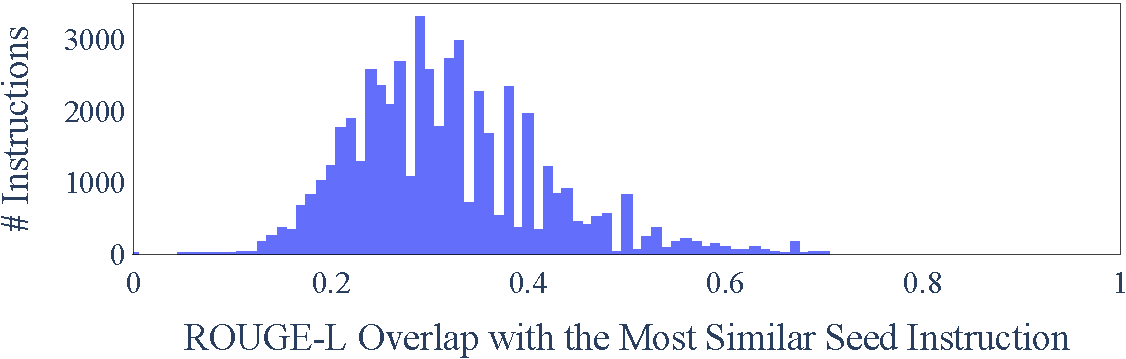
\includegraphics[width=\linewidth]{figures/overlap_with_seed_instructions.pdf}
    \end{subfigure}
    \caption{Distribution of the ROUGE-L scores between generated instructions and their most similar seed instructions. \label{fig:overlap-distribution}}
    \par\bigskip
    \begin{subfigure}{0.99\linewidth}
      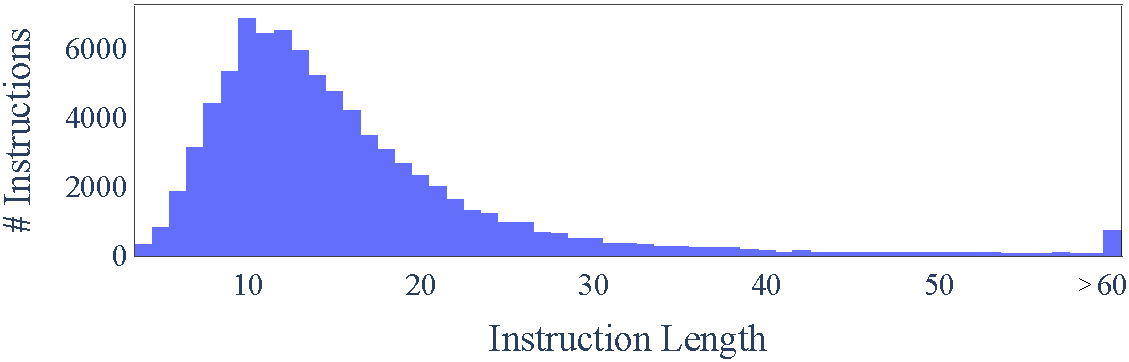
\includegraphics[width=\linewidth]{figures/instruction_length.pdf}
    \end{subfigure}
    \par\medskip
    \begin{subfigure}{0.99\linewidth}
      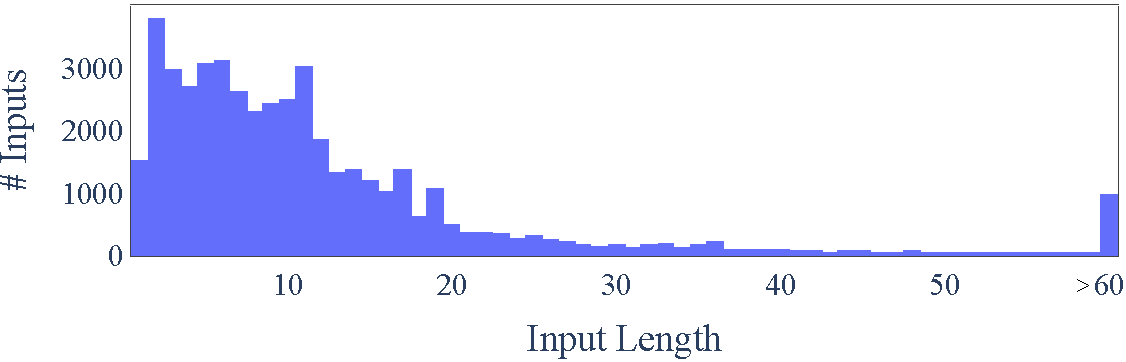
\includegraphics[width=\linewidth]{figures/input_length.pdf}
    \end{subfigure}
    \par\medskip
    \begin{subfigure}{0.99\linewidth}
      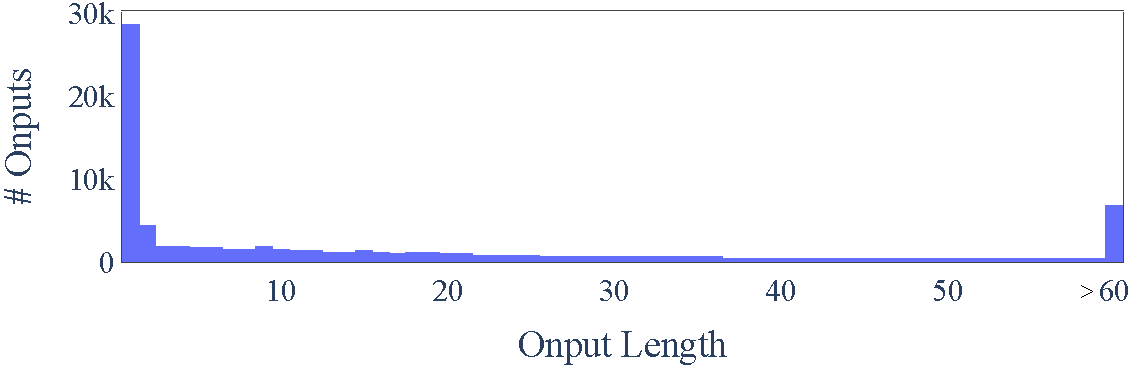
\includegraphics[width=\linewidth]{figures/output_length.pdf}
    \end{subfigure}
    \caption{Length distribution of the generated instructions, non-empty inputs, and outputs.  \label{fig:length_distribution}
  }
  \end{minipage}
  }

\end{figure*}